\begin{boxnote}
      \begin{description}
        \item[種類] Rapid commuunications
        \item[閲覧日] 24th May 2025
        \item[キーワード] EIT, OMIT
        \item[文献番号] \cite{PhysRevA.81.041803}
        \item[関連論文] \Lambda 型エネルギーのEIT\cite{PhysRevLett.84.5094}, 実験実証\cite{science.1195596}
      \end{description}
    \end{boxnote}
    \section{行ったこと}
      オプトメカニクス系におけるElectromagnetically induced transparency (EIT),OMITを予言した.
    \section{原理}
      系のハミルトニアンを,
      \begin{align}
        \hat{H} = \hbar\omega_0\hat{c}^{\dag}\hat{c} + \qty(\frac{\hat{p}^2}{2m} + \frac{1}{2}m\omega^2_{\r{m}}\hat{q}^2) + \i\hbar\epsilon_{\r{c}}\qty(\hat{c}^{\dag}\e^{-\i\omega_{\r{c}}t} - \hat{c}\e^{\i\omega_{\r{c}}t}) + \i\hbar\qty(\hat{c}^{\dag}\epsilon_{\r{p}}\e^{-\i\omega_{\r{p}}t} - \hat{c}\epsilon^*_{\r{p}}\e^{\i\omega_{\r{p}}t}) - \chi_0\hat{c}^{\dag}\hat{c}\hat{q}
      \end{align}
      とする.
      $\hat{c}$は共振器内光子の消滅演算子,$\hat{q}$, $\hat{p}$は共振器の振動に関する量子化した位置と運動量,$\epsilon_{\r{c}}$はポンプ光のエネルギー,$\epsilon_{\r{p}}$はプローブ光のエネルギーである.
      なお,結合定数$\chi_0 = \hbar\omega_0 / L$において,$L$は共振器長である.
      系のセットアップは\reff{PhysRevA.81.041803-fig-1}の通り.
      \begin{figure}[H]
        \centering
        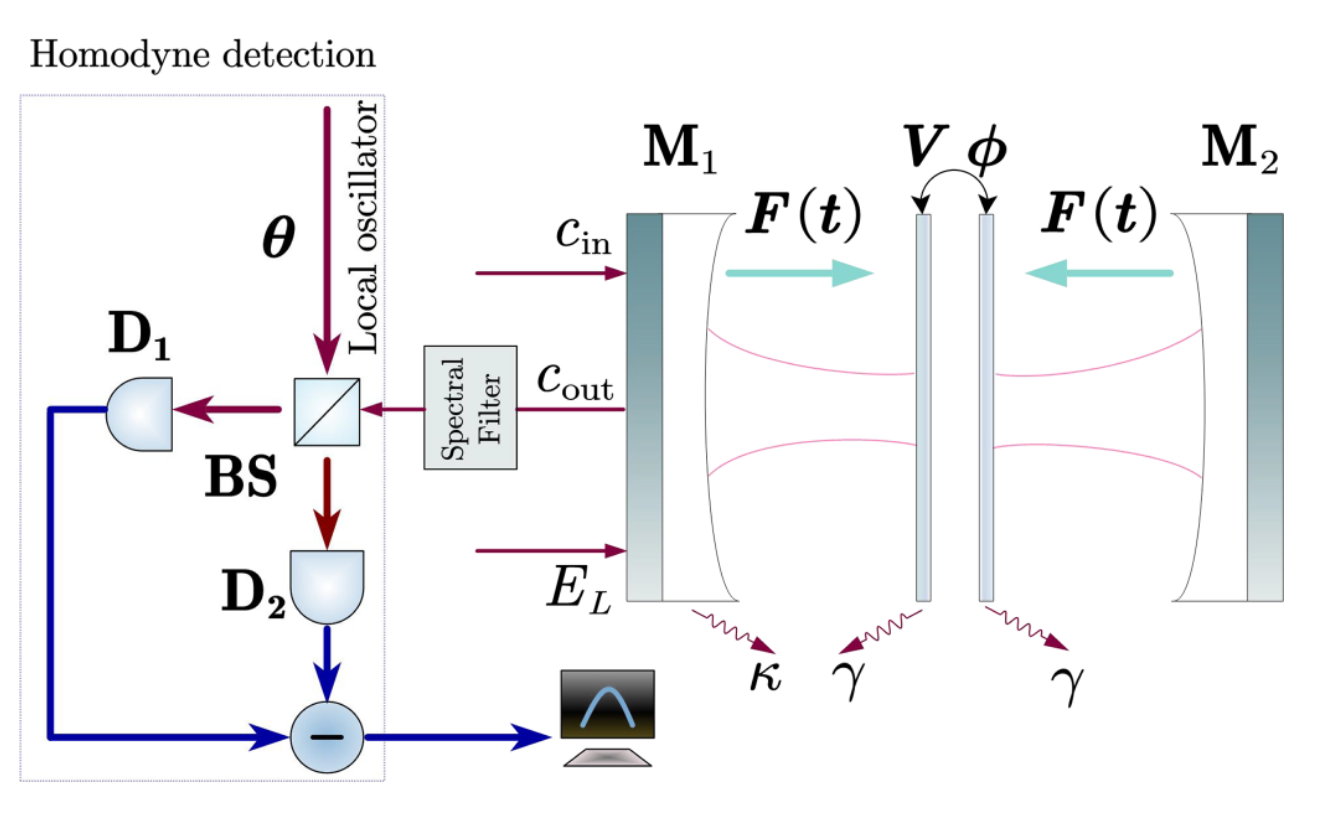
\includegraphics[width = 0.5\linewidth]{/home/hawk/desktop/lab/papers/src/Electromagnetically_induced_transparency_in_mechanical_effects_of_light/1.png}
        \caption{系のセットアップ}\label{PhysRevA.81.041803-fig-1}
      \end{figure}
      演算子,$\hat{q}$,$\hat{p}$,$\hat{c}$の時間発展を考える.
      ただし,
      \begin{align}
        \qty[\hat{q}, \hat{p}] = \i\hbar,\quad \qty[\hat{c}, \hat{c}^{\dag}] = 1
      \end{align}
      である.
      \begin{align}
        \dv{\hat{q}}{t} =& -\frac{\i}{\hbar}\qty[\hat{q}, \hat{H}] \\ 
        =& -\frac{\i}{\hbar}\qty[\hat{q}, \frac{\hat{p}^2}{2m}] \\ 
        =& \frac{\hat{p}}{m}, \\ 
        \dv{\hat{p}}{t} =& -\frac{\i}{\hbar}\qty[\hat{p}, \hat{H}] \\ 
        =& -\frac{\i}{\hbar}\qty[\hat{p}, \frac{1}{2}m\omega^2_{\r{m}}\hat{q}^2] + \frac{\i}{\hbar}\chi_0\hat{c}^{\dag}\hat{c}\qty[\hat{p}, \hat{q}] \\ 
        =& -m\omega^2_{\r{m}}\hat{q} + \chi_0\hat{c}^{\dag}\hat{c}, \label{PhysRevA.81.041803-eom-p} \\ 
        \dv{\hat{c}}{t} =& -\frac{\i}{\hbar}\qty[\hat{c}, \hat{H}] \\ 
        =& -\frac{\i}{\hbar}\qty[\hat{c}, \hbar\omega_0\hat{c}^{\dag}\hat{c}] - \frac{\i}{\hbar}\qty[\hat{c}^{\dag}, \i\hbar\epsilon_{\r{c}}\hat{c}^{\dag}\e^{-\i\omega_{\r{c}}t}] - \frac{\i}{\hbar}\qty[\hat{c}^{\dag}, \i\hbar\hat{c}^{\dag}\epsilon_{\r{p}}\e^{-\i\omega_{\r{p}}t}] - \frac{\i}{\hbar}\qty[\hat{c}, \chi_0\hat{c}^{\dag}\hat{c}]\hat{q} \\ 
        =& -\i\omega_0\hat{c} + \epsilon_{\r{c}}\e^{-\i\omega_{\r{c}}t} + \epsilon_{\r{p}}\e^{-\i\omega_{\r{p}}t} + \frac{\i}{\hbar}\chi_0\hat{c}\hat{q}\label{PhysRevA.81.041803-eom-c-1}.
      \end{align}
      \refe{PhysRevA.81.041803-eom-c-1}については,周波数$\omega_{\r{c}}$で回転する座標で見ると,$\hat{c} = \tilde{c}\e^{-\i\omega_{\r{c}}t}$とすればよく,
      \begin{align}
        \dv{\tilde{c}}{t} = \i\omega_{\r{c}}\tilde{c} - \i\qty(\omega_0 - \chi_0\hat{q})\tilde{c} + \epsilon_{\r{c}} + \epsilon_{\r{p}}\e^{\i\qty(\omega_{\r{c}} - \omega_{\r{p}}t)} \label{PhysRevA.81.041803-eom-c-2}
      \end{align}
      となる.
      期待値を取る.
      さらに,恣意的にダンピング項を入れる.
      すなわち,\refe{PhysRevA.81.041803-eom-p}の右辺に$-\gamma\hat{p}$を足し,\refe{PhysRevA.81.041803-eom-c-2}の右辺に$-\kappa\tilde{c}$を足す.
      まとめると,
      \begin{align}
        \dv{\hat{q}}{t} =& \frac{\ev{\hat{p}}}{m}, \label{PhysRevA.81.041803-eom-q-ev} \\ 
        \dv{\hat{p}}{t} =& -m\omega^2_{\r{m}}\ev{\hat{q}} + \chi_0\ev{\tilde{c}^{\dag}}\ev{\tilde{c}} - \gamma_{\r{m}}\ev{\hat{p}}, \label{PhysRevA.81.041803-eom-p-ev} \\ 
        \dv{\tilde{c}}{t} =& -\qty[\kappa + \i\qty(\omega_0 - \omega_{\r{c}} - \frac{\chi_0}{\hbar}\ev{\hat{q}})]\ev{\tilde{c}} + \epsilon_{\r{c}} + \epsilon_{\r{p}}\e^{\i\qty(\omega_{\r{c}} - \omega_{\r{p}}t)} \label{PhysRevA.81.041803-eom-c-ev}.
      \end{align}
      また,光子の入出力関係から,
      \begin{align}
        \epsilon_{\r{out}}(t) + \epsilon_{\r{p}}\e^{-\i\omega_{\r{p}}t} + \epsilon_{\r{c}}\e^{-\i\omega_{\r{c}}t} = 2\kappa\ev{\hat{c}} \label{PhysRevA.81.041803-io-relation}
      \end{align}
      が成立する.
      さて,ポンプ光が存在しないときの入出力関係式を考える.
      $\epsilon_{\r{c}} = 0$とすると,\refe{PhysRevA.81.041803-io-relation}は,
      \begin{align}
        \epsilon_{\r{out}}(t) + \epsilon_{\r{p}}\e^{-\i\omega_{\r{p}}t} = 2\kappa\ev{\hat{c}}
      \end{align}
      となる.
      なお,$\ev{\hat{c}}$の時間変化は\refe{PhysRevA.81.041803-eom-c-ev}ではなく,\refe{PhysRevA.81.041803-eom-c-1}を用いて,
      \begin{align}
        \ev{\dv{\hat{c}}{t}} = -\qty[\kappa + \i\qty(\omega_0 - \frac{\chi_0}{\hbar}\ev{\hat{q}})]\ev{\hat{c}} + \epsilon_{\r{p}}\e^{-\i\omega_{\r{p}}t}
      \end{align}
      と書き換えられる.
      ポンプ光が存在しないとき,可動鏡の平均位置はプローブ光による変位であるから,
      \begin{align}
        \ev{\hat{q}} = L\frac{\hbar\omega_{\r{p}}}{\hbar\omega_0} = L\frac{\omega_{\r{p}}}{\omega_0} = \frac{\hbar\omega_{\r{p}}}{\chi_0}
      \end{align}
      となる.
      また,定常状態について考えれば,
      \begin{align}
        \ev{\dv{\hat{c}}{t}} = 0.
      \end{align}
      結局,
      \begin{align}
        \ev{\hat{c}} = \frac{\epsilon_{\r{p}}\e^{-\i\omega_{\r{p}}t}}{\kappa + \i\qty(\omega_0 - \omega_{\r{p}})}
      \end{align}
      となる.
      これを用いると,共振器内の平均光子数を入力,外部の光子数を出力とした伝達函数を考えることができる.
      特に,プローブ光の周波数での応答を考えたいので,
      \begin{align}
        \epsilon_{\r{T}} = \frac{2\kappa\ev{\hat{c}}}{\epsilon_{\r{p}}\e^{-\i\omega_{\r{p}}t}}
      \end{align}
      を伝達函数とする.
      もちろん,ポンプ光が存在しないときは,
      \begin{align}
        \epsilon_{\r{T}} = \frac{1}{\kappa + \i\qty(\omega_0 - \omega_{\r{p}})}
      \end{align}
      である.
      ポンプ光が存在するときの伝達函数について求めることは出来なかったが,論文では行われており,
      \begin{align}
        \epsilon_{\r{T}} = \frac{2\kappa}{d(\delta)}\qty[\qty(\delta^2 - \omega^2_{\r{m}} + \i\gamma_{\r{m}}\delta)\qty(\kappa - \i\qty(\Delta + \delta)) - 2\i\omega_{\r{m}}\beta] \\ 
      \end{align}
      where,
      \begin{align}
        d(\delta) \coloneqq& \qty(\delta^2 - \omega^2_{\r{m}} + \i\gamma_{\r{m}})\qty(\qty(\kappa - \i\delta)^2 + \Delta^2) + 4\Delta\omega_{\r{m}}\beta, \\ 
        \delta \coloneqq& \omega_{\r{p}} - \omega_{\r{c}}, \\ 
        \Delta \coloneqq& \omega_0 - \omega_{\r{c}} - \frac{2\beta\chi_0}{\omega_{\r{m}}}, \\ 
        \beta \coloneqq& \frac{\chi^2_0\abs{\tilde{c}_0}^2}{2m\hbar\omega_{\r{m}}}, \\ 
        \tilde{c}_0 \coloneqq& \frac{\epsilon_{\r{c}}}{\kappa + \i\Delta}.
      \end{align}
      おそらくここがこの論文の革新的な仕事なのだろう.
      伝達函数の実部を$\mathcal{V}_{\r{p}}$,虚部を$\tilde{\mathcal{V}}_{\r{p}}$とする.
      伝達函数を,
      \begin{align}
        \epsilon_{\r{T}} = \frac{A_+}{x - x_+} + \frac{A_-}{x - x_-} \label{PhysRevA.81.041803-trans}
      \end{align}
      と書く.
      実部は,出力光の強度,虚部は位相を表す.
      \begin{figure}[H]
        \centering
        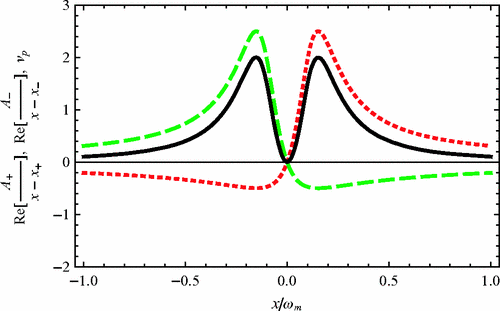
\includegraphics[width = 0.5\linewidth]{/home/hawk/desktop/lab/papers/src/Electromagnetically_induced_transparency_in_mechanical_effects_of_light/4.png}
        \caption{黒が伝達函数の実部.赤が\refe{PhysRevA.81.041803-trans}の第1項の実部,赤が第2項の実部.}
      \end{figure}
      \begin{figure}[H]
        \centering
        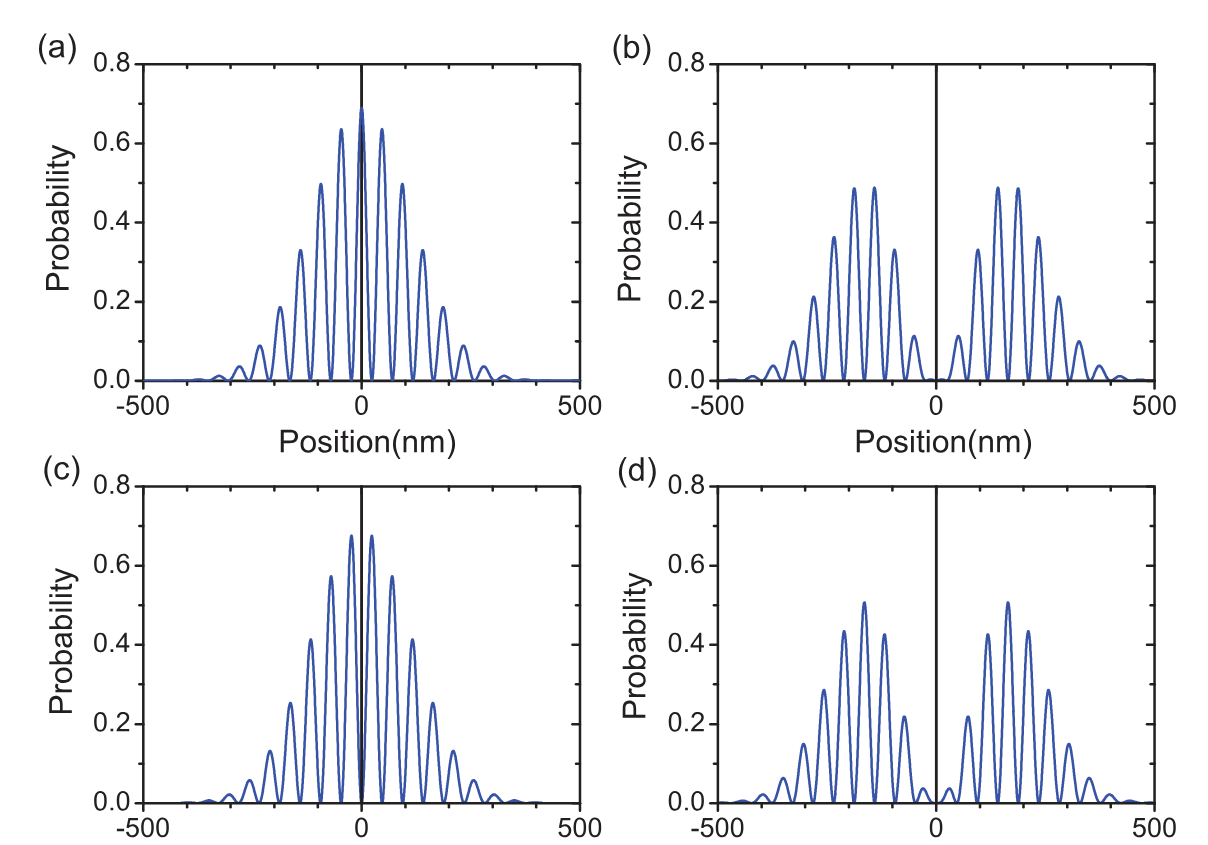
\includegraphics[width = 0.5\linewidth]{/home/hawk/desktop/lab/papers/src/Electromagnetically_induced_transparency_in_mechanical_effects_of_light/5.png}
        \caption{黒が伝達函数の虚部.赤が\refe{PhysRevA.81.041803-trans}の第1項の虚部,赤が第2項の虚部.}
      \end{figure}